%%%%%%%%%%%%%%%%%%%%%%%%%%%%%%%%%%%%%%%%%%%%%%%%%%%%%%%%%%%%%%%%%%%%%%%%%%%%%%%%%%%%
% Do not alter this block (unless you're familiar with LaTeX
\documentclass{article}
\usepackage[margin=1in]{geometry} 
\usepackage{amsmath,amsthm,amssymb,amsfonts, fancyhdr, color, comment, graphicx, environ}
\usepackage{xcolor}
\usepackage{mdframed}
\usepackage{float}
\usepackage[shortlabels]{enumitem}
\usepackage{indentfirst}
\usepackage{physics}
\usepackage{hyperref}
\usepackage{sectsty}
\usepackage{longtable}
\usepackage{complexity}
\sectionfont{\fontsize{12}{15}\selectfont}
\newcommand{\powerset}{\raisebox{.15\baselineskip}{\Large\ensuremath{\wp}}}
\usepackage{tikz}

\usetikzlibrary{arrows,shapes.gates.logic.US,shapes.gates.logic.IEC,calc,decorations.pathmorphing}
\tikzset{snake it/.style={decorate, decoration=snake}}

\usepackage{subcaption}
\usepackage{amsfonts}
\usepackage{lipsum}
\usepackage{setspace}
\usepackage[qm]{qcircuit}
\usepackage[mmddyy]{datetime}
\usepackage{mathtools}
\DeclarePairedDelimiter\ceil{\lceil}{\rceil}
\DeclarePairedDelimiter\floor{\lfloor}{\rfloor}
\usepackage{tkz-euclide}
\usepackage{wasysym}
\hypersetup{
    colorlinks=true,
    linkcolor=blue,
    filecolor=magenta,      
    urlcolor=blue,
}


\makeatletter
\renewcommand*\env@matrix[1][*\c@MaxMatrixCols c]{%
  \hskip -\arraycolsep
  \let\@ifnextchar\new@ifnextchar
  \array{#1}}
\makeatother

\definecolor{lightgray}{rgb}{0.83, 0.83, 0.83}
\pagestyle{fancy}

\def\centerarc[#1](#2)(#3:#4:#5)% Syntax: [draw options] (center) (initial angle:final angle:radius)
    { \draw[#1] ($(#2)+({#5*cos(#3)},{#5*sin(#3)})$) arc (#3:#4:#5); }

\newcommand*\unit[1]{\mathbf{\hat{{#1}}}}

\newcommand\avg[1]{\langle #1 \rangle}

\newenvironment{problem}[2][Problem]
    { \begin{mdframed}[backgroundcolor=gray!20] \textbf{#1 #2} \\}
    {  \end{mdframed}}

% Define solution environment
\newenvironment{solution}{\noindent \textbf{Solution}\\}

% \begin{mdframed}[backgroundcolor=gray!20, align = center, userdefinedwidth = 3.8in]
%     \includegraphics[width = 3.5in]{5C_HW5_Img2.png}
% \end{mdframed}

    
%%%%%%%%%%%%%%%%%%%%%%%%%%%%%%%%%%%%%%%%%%%%%
%Fill in the appropriate information below 
\lhead{Thomas Lu}
\chead{\textbf{Signal Generator Notes}}
%%%%%%%%%%%%%%%%%%%%%%%%%%%%%%%%%%%%%%%%%%%%%


\begin{document}
    \section*{Fri 2/23}
    \subsection*{Function generator general explorations}
    Using the built-in controls of the function generator (AFG), I generated waveforms using the built-in menu options (e.g. sine, square, pulse,) and displayed the signals on the oscilloscope. I also familiarized myself with the various functions and controls on the oscilloscope and AFG.
    \subsubsection*{Phase difference due to cables}
    Both channels on the AFG were set to 6MHz, 200m$V_{pp},$ with a phase offset of $0,$ and were connected to channels 1 and 2 on the oscilloscope. Even after the "Align Phase" option on the AFG is enabled, the oscilloscope still shows a slight phase difference: 
    \begin{mdframed}[backgroundcolor=gray!20, align = center, userdefinedwidth = 3.8in]
    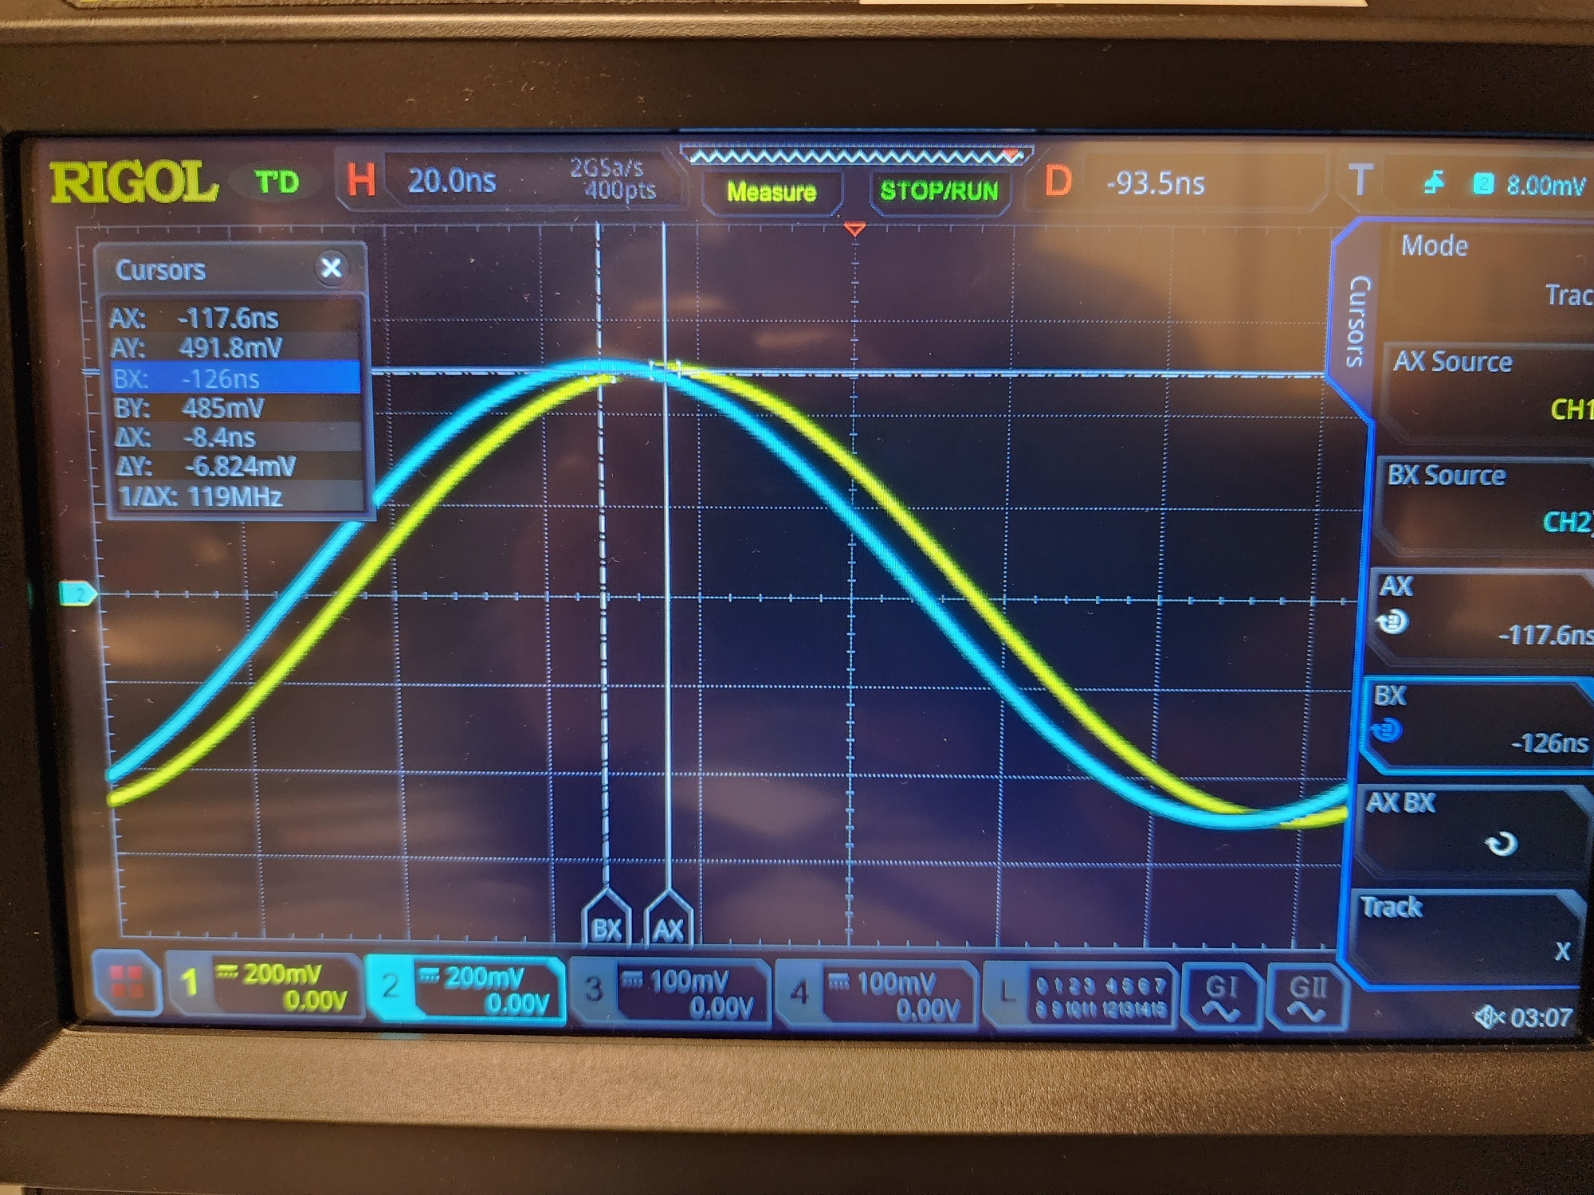
\includegraphics[width = 3.5in]{img/phase_difference.jpg}
    \\Peak-to-peak difference of 8.4ns between CH1 (yellow) and CH2 (blue)
    \end{mdframed}
    Most likely, this is due to the difference in wire lengths, as the CH2 wire was 70cm, while the CH1 wire was 210cm long. We can use this to calculate the speed of the signal:
    $$v = \frac{\Delta \ell}{\Delta t} = \frac{140cm}{8.4ns} \approx 0.55c$$
    which seems reasonable for electrons in copper
    \subsection*{Programming the function generator with a computer}
    Useful resources:
    \begin{itemize}
    \item \href{https://acidbourbon.wordpress.com/2019/09/12/send-numpy-data-to-rigol-dg4202-arbitrary-waveform-generator-via-lan/}{Example using LAN and Python}
    \item \href{https://www.eevblog.com/forum/testgear/dg4000dg4162-scpi-arbitrary-waveform-programming/}{General info about programming}
    \item \href{https://www.eevblog.com/forum/testgear/dg4000-a-firmware-investigation/}{Deeper dive into firmware}
    \end{itemize}
    A script for 
\end{document}